\documentclass[journal,12pt,twocolumn]{IEEEtran}
\usepackage{graphicx, float}
\graphicspath{{./figs/}}{}
\usepackage{amsmath,amssymb,amsfonts,amsthm}
\newcommand{\myvec}[1]{\ensuremath{\begin{pmatrix}#1\end{pmatrix}}}
\usepackage{tabularx}
\usepackage{circuitikz}
\usetikzlibrary{calc}
\usepackage{enumitem}
\usepackage{listings}
\usepackage{watermark}
\usepackage{titlesec}
\let\vec\mathbf
\lstset{
frame=single, 
breaklines=true,
columns=fullflexible
}

\title{\mytitle}
\title{
8x1 MUX logic in ARM
}
\author{Pratheek Darla}
\date{October 2022}

\begin{document}
\maketitle
\tableofcontents
\bigskip


\section{\textbf{Abstract}}
The objective of this manual is to show how to implement the Boolean function -
\begin{equation}
Q = B.C + A.B.D' + A'.C'.D   \label{eq-1}
\end{equation}
in ARM.

\begin{center}
    
\vspace{10mm}    

 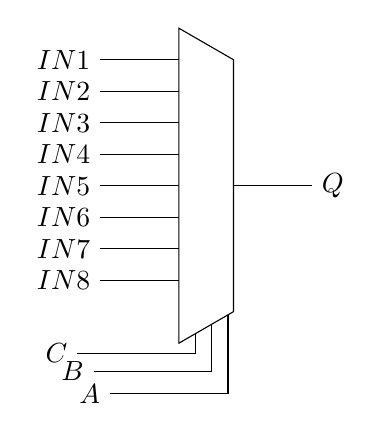
\begin{tikzpicture}

    \draw[scale=0.8] 
                (90,8)coordinate (O)
            --++(30:1)coordinate (A)
            --++(90:4)coordinate (B)
            --++(150:1) coordinate (C)
            --cycle;
        \draw ($(A)!0.5!(B)$)--++(0:1)node[right]{$Q$};

    \draw ($(O)!0.9!(A)$)--++(-90:1)--++(180:1.5)node[left]{$A$};

    \draw ($(O)!0.3!(A)$)--++(-90:0.25)--++(180:1.5)node[left]{$C$};
    \draw ($(O)!0.6!(A)$)--++(-90:0.6)--++(180:1.5)node[left]{$B$};

    \foreach \y/\t in {0.1/1,0.2/2,0.3/3,0.4/4,0.5/5,0.6/6,0.7/7,0.8/8} {
    \draw ($(C)! \y*1 !(O)$)--++(180:1) node[left] {$IN \t$};}      

    \end{tikzpicture}
    \\ Figure- 8:1 multiplexer
\end{center}


\begin{circuitikz} \draw

(0,14) node[and port,number inputs=4]  (and1) {}
(0,12) node[and port,number inputs=4]  (and2) {}
(0,10) node[and port,number inputs=4]  (and3) {}
(0,8) node[and port,number inputs=4]  (and4) {}
(0,6) node[and port,number inputs=4]  (and5) {}
(0,4) node[and port,number inputs=4]  (and6) {}
(0,2) node[and port,number inputs=4]  (and7) {}
(0,0) node[and port,number inputs=4]  (and8) {}
(4.5,7) node[or port, number inputs=8] (or) {}
(and1.out) -- (or.in 1)
(and2.out) -- (or.in 2)
(and3.out) -- (or.in 3)
(and4.out) -- (or.in 4)
(and5.out) -- (or.in 5)
(and6.out) -- (or.in 6)
(and7.out) -- (or.in 7)
(and8.out) -- (or.in 8);
\node[left] at (and1.in 1) {\(D\)};
\node[left] at (and1.in 2) {\(A\)};
\node[left] at (and1.in 3) {\(B\)};
\node[left] at (and1.in 4) {\(C\)};
\node[left] at (and1.in 2)[ocirc] {};
\node[left] at (and1.in 3)[ocirc] {};
\node[left] at (and2.in 1) {\(0\)};
\node[left] at (and2.in 2) {\(A\)};
\node[left] at (and2.in 3) {\(B\)};
\node[left] at (and2.in 4) {\(C\)};
\node[left] at (and2.in 2)[ocirc] {};
\node[left] at (and3.in 1) {\(D\)};
\node[left] at (and3.in 2) {\(A\)};
\node[left] at (and3.in 3) {\(B\)};
\node[left] at (and3.in 4) {\(C\)};
\node[left] at (and3.in 3)[ocirc] {};
\node[left] at (and4.in 1) {\(D'\)};
\node[left] at (and4.in 2) {\(A\)};
\node[left] at (and4.in 3) {\(B\)};
\node[left] at (and4.in 4) {\(C\)};
\node[right] at (or.out) {\(Q(Output)\)};
\node[left] at (and5.in 1) {\(0\)};
\node[left] at (and5.in 2) {\(A\)};
\node[left] at (and5.in 3) {\(B\)};
\node[left] at (and5.in 4) {\(C\)};
\node[right] at (or.out) {\(Q(Output)\)};
\node[left] at (and6.in 1) {\(0\)};
\node[left] at (and6.in 2) {\(A\)};
\node[left] at (and6.in 3) {\(B\)};
\node[left] at (and6.in 4) {\(C\)};
\node[right] at (or.out) {\(Q(Output)\)};
\node[left] at (and7.in 1) {\(1\)};
\node[left] at (and7.in 2) {\(A\)};
\node[left] at (and7.in 3) {\(B\)};
\node[left] at (and7.in 4) {\(C\)};
\node[right] at (or.out) {\(Q(Output)\)};
\node[left] at (and8.in 1) {\(1\)};
\node[left] at (and8.in 2) {\(A\)};
\node[left] at (and8.in 3) {\(B\)};
\node[left] at (and8.in 4) {\(C\)};
\node[right] at (or.out) {\(Q(Output)\)};
\end{circuitikz}
\begin{center}
 Figure- Logic circuit for the given boolean function
\end{center}

\section{\textbf{Components}}
  \begin{tabularx}{0.48\textwidth} { 
  | >{\centering\arraybackslash}X 
  | >{\centering\arraybackslash}X 
  | >{\centering\arraybackslash}X | }
\hline
 \textbf{Components}& \textbf{Values} & \textbf{Quantity}\\
\hline
Vaman Board &  & 1 \\  
\hline
JumperWires& M-F & 5 \\ 
\hline
Breadboard &  & 1 \\
\hline
USB-C cable&  & 1 \\
\hline
\end{tabularx}

\begin{center}
    Table- Components
\end{center}

\section{Setup}
\begin{enumerate}
\item Connect the Vaman to the Laptop through USB.
\item There is a button and an LED to the left of the USB port on the Vaman.There is another button to the right of the LED.
\item Press the right button first and immediately press the left button. The LED will be blinking green. The Vaman is now in bootloader mode.
\end{enumerate}

\section{Implementation}

The code below realizes the Boolean logic for Q in (\ref{eq-1})  using 5V,GND  pins of Vaman Board.
\\
2,4,6,8 GPIO Pins of Vaman Board are configured as input pins and the required Logic for A, B, C, D are drawn from 5V (Digital '1'), GND (Digital '0'). Built in led at 22nd pin will glow based on Q satisfying the Table-2.

\begin{lstlisting}
https://github.com/PratheekDarla/FWC-IITH/trunk/arm/codes/src/main.c
\end{lstlisting}


\vspace{5mm}    

\begin{tabularx}{0.50\textwidth} { 
  | >{\centering\arraybackslash}X
  | >{\centering\arraybackslash}X 
  | >{\centering\arraybackslash}X 
  || >{\centering\arraybackslash}X 
  | >{\centering\arraybackslash}X 
  | >{\centering\arraybackslash}X| }
\hline
Selection
line&Selection
line&Selection line&Input &Output\\
\hline
C&  B & A & D & Q\\
\hline
0 & 0 & 0 & D & D\\  
\hline
0 & 0 & 1 & 0 & 0\\ 
\hline
0 & 1 & 0 & D & D\\
\hline
0 & 1 & 1 & D' & D'\\
\hline
1 & 0 & 0 & 0 & 0\\
\hline
1 & 0 & 1 & 0 & 0\\
\hline
1 & 1 & 0 & 1 & 1\\
\hline
1 & 1 & 1 & 1 & 1\\
\hline
\end{tabularx}

\vspace{5mm}    

\begin{enumerate}
\item Login to termux-ubuntu on the android device and execute the following commands:\\
Make sure that the required installation of pygmy-sdk had done prior executing below commands
\begin{lstlisting}
proot-distro login debian
cd  /data/data/com.termux/files/home/
mkdir arm
svn co https://github.com/PratheekDarla/FWC-IITH/trunk/arm/codes
\end{lstlisting}
\begin{lstlisting}
cd codes/GCC_Project
make
scp /data/data/com.termux/files/home/arm/codes/GCC_Project/output/bin/codes.bin usernameofpc@IPaddress:/home/username
\end{lstlisting}
Make sure that the appropriate username, IP address of the Laptop is given in the above command.
\item Now execute the following commands on the Laptop terminal.\\
Make sure that required installation of programmer application and modification of bash file had done prior executing below command
\begin{lstlisting}
bash flash.sh codes.bin
\end{lstlisting}
\item After finishing the process of flashing with the programmer application press the button to the right of the USB port to reset. Vaman is now flashed with our source code.
\end{enumerate}


\end{document}